
%%%%%%%%%%%%%%%%%%%%%%%%%%%%%%%%%%%%%%%%%%%%%%%%%%%%%%%%%%%%%%%%%%%%%%%%
\chapter{Introduction}  \label{introduction}
%%%%%%%%%%%%%%%%%%%%%%%%%%%%%%%%%%%%%%%%%%%%%%%%%%%%%%%%%%%%%%%%%%%%%%%%

\begin{center}
  \begin{minipage}{0.5\textwidth}
    \begin{small}
      "Some say the world will end in fire, some say in ice." 
      
      ― Robert Frost
    \end{small}
  \end{minipage}
  \vspace{0.5cm}
\end{center}

\noindent Though the world knows by now that global climate change is a practically unstoppable force that will eventually dramatically affect humanity and our world, exactly how it affects this future is not known yet. Is a widely documented and proven phenomena, the resultant effects of it on the natural world that we inhabit is still an ongoing mystery, but one that can be investigated in the present. 

%%%%%%%%%%%%%%%%%%%%%%%%%%%%%%%%%%%%%%%%%%%%%%%%%%%%%%%%%%%%%%%%%%%%%%%%
\section{The Arctic Environment and the Beaufort Duct} \label{intro_enviro}
%%%%%%%%%%%%%%%%%%%%%%%%%%%%%%%%%%%%%%%%%%%%%%%%%%%%%%%%%%%%%%%%%%%%%%%%

In the Arctic, where the effects of climate change are felt harder due to the ice albedo effect in a positive feedback look, these long term effects of global scale climate change have been observed sooner. In particular, the warming polar basin has decreased the coverage, length, and thickness of the Arctic ice sheet dramatically, resulting in the loss of thick multi-year ice that used to last through the summer. The Canada basin, from which the data for this project originated, has seen drastic decreases in the ice pack even when compared to the rest of the impacted Arctic, making it a critical area of study. \footcite[]{mclaughlin2011rapid}

Since the 1970's the increase of melting ice has allowed for the movement of warmer water from the pacific to enter the Arctic Basin. This has created a new acoustic phenomena known as the Beaufort duct \footcite[]{toole2010influences}. Situated around 300 m of depth, this duct conducts sound in a deeper channel not formerly seen in the Arctic environment. The duct also opens up the potential for more deeper water, long range underwater communications, leading to much interest in its properties. The decrease of ice coverage also comes with an increase in anthropogenic activity as the opening of the arctic passageway leads to more anthropologically generated noise, including shipping, drilling, and recreation. \footcite[]{judson2010trends} The shrinking ice and intrusion of human activities is already known to change the behavior of some fish, which affects the ecosystem of the Arctic as a whole. \footcite[]{ivanova2020shipping}.

The Canada Basin Acoustic Propagation Experiment (CANAPE) was an operation designed to focus on sound within the Beaufort Duct in order to gain more knowledge about its effects. With the current trends in climate change and the permanently warmer arctic, the duct can be found nearly all year \footcite[]{duda2017acoustic}, making its effects more perennial than before. As reversing climate change seems unlikely and ice-less summers loom on the horizon \footcite[]{notz2020}, the Beaufort Duct has become an almost permanent fixture of the Arctic soundscape. Therefore, studying its effects on ambient noise will help predict the possible implications of this climate phenomena on the Arctic and its spreading effects on humans, biologic life, and more.



%%%%%%%%%%%%%%%%%%%%%%%%%%%%%%%%%%%%%%%%%%%%%%%%%%%%%%%%%%%%%%%%%%%%%%%%
\subsection{Noise in the Arctic}    \label{intro_arctic_noise}
%%%%%%%%%%%%%%%%%%%%%%%%%%%%%%%%%%%%%%%%%%%%%%%%%%%%%%%%%%%%%%%%%%%%%%%%

Typically, sound in water travels three times faster than it does in air, a rough comparison of 1500 m/s (water) to 343 m/s (air). Underwater, sound curves towards lower speeds, trapping much low-angle sound in the duct. \footcite[]{chen2020tempo}  Because of this, the appeal of underwater acoustic operations has added much research into areas of navigation, communication, and other uses of the duct. Various interests lie in research into the Beaufort duct, from its effects on biology in the region to economic and political exploitation. 

The speed of sound in water is affected by a variety of factors, including temperature, salinity, and pressure. Before, the runoff of freshwater from the ice sheet melt created a warm water layer which acted as a shallow surface duct with an increasing gradient to the bottom. The effects of climate change on the Arctic have made major changes to the temperature profile under the ice, resulting in a different Arctic sound speed profile. The new Arctic sound speed profile has two ducts, the original surface, and the deeper Beaufort Duct. This sound speed profile in \autoref{fig_ssp} was taken during the operations of CANAPE and shows the clear presence of the Beaufort Duct through multiple time periods. \footcite[]{Bonnel2021} 

\begin{figure}[ht]
\centering
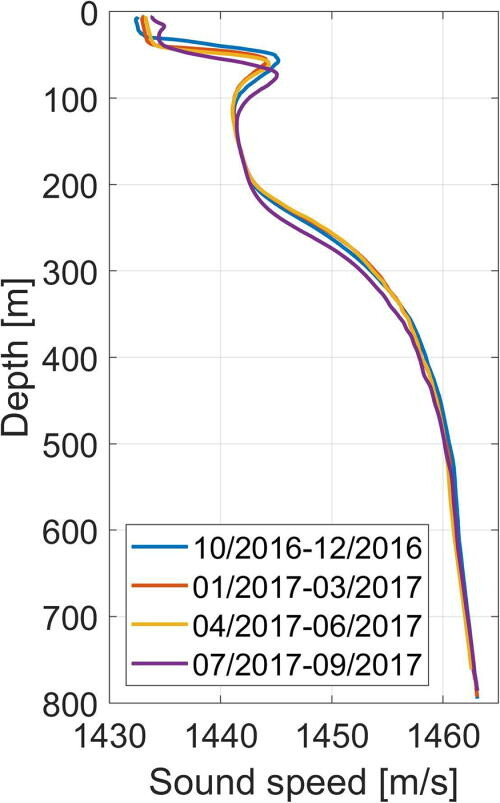
\includegraphics[scale=2]{Figures/ssp.jpeg}
\caption{Sound speed profiles in the Chukchi sea displaying presence of Beaufort duct. Image reproduced with author's permission}
\label{fig_ssp}
\end{figure}

Ambient noise is typically comprised of all the living and nonliving factors generating noise in an environment, essentially the base level of an environment. Underwater, this sound is normally produced at the surface through wind, waves, and precipitation; a portion also comes from geological processes at the sea floor \footcite[]{dziak2015sources}. Marine life communication \footcite[]{ladegaard2021} and anthropogenic operations also contributes to this noise level. In the Arctic, the presence of ice removes air-sea interactions and replaces them with ice driven noise. From icequakes\footcite[]{muller2005singing} and vibrations\footcite[]{kinda2015arctic}, to calving \footcite[]{matsumoto2014antarctic}, cracking\footcite[]{milne1964ambient}, and melting     \footcite[]{glowacki2018intensity} \footcite[]{mahanty2020melt}, ice generates plenty of underwater ambient noise. 

%%%%%%%%%%%%%%%%%%%%%%%%%%%%%%%%%%%%%%%%%%%%%%%%%%%%%%%%%%%%%%
\section{The CANAPE Experiment} \label{intro_canape}

The Canada Basin Acoustic Propagation Experiment (CANAPE) was a yearlong acoustic recording operation conducted from 2016 to 2017 in the Chukchi Sea and Shelf as part of a investigation conducted by the Woods Hole Oceanographic Institution (WHOI) into the Beaufort Duct. There were two facets to this experiment, the deep water Canada Basin (DW-CANAPE) and the shallower water Chukchi Shelf (SW-CANAPE) \footcite[]{ballard2020yearlong}. The acoustic data for this thesis specifically comes from SW-CANAPE.

For SW-CANAPE an array was deployed at the site as seen in \autoref{fig_location}. The specific locations and depths can be seen in \autoref{table_location} It consisted of five several hydrophone recording units (SHRU(s)). Each SHRU had four channels in a vertical line array and also contained temperature and pressure sensors. These channels were deliberatly placed at the depth of the Beaufort Duct to amplify its effects. Data from SHRU1 and SHRU5 are used in this analysis.

\begin{table}
  \centering
  \begin{tabular}{|| c c c c||}
    \toprule
    \textbf{SHRU}  & \textbf{Latitude N}  & \textbf{Longitude W}  & \textbf{Water Depth m}\\
    \midrule
      \texttt{WHOI SHRU 1}  & 72° 54.4123’ & 159° 01.0840’ & 302 \\
      \texttt{WHOI SHRU 2}  & 72° 45.2347’ & 158° 16.3243’ & 308 \\
      \texttt{WHOI SHRU 3}  & 72° 40.6924’ & 157° 54.6493’ & 303 \\
      \texttt{WHOI SHRU 4}  & 72° 36.6582’ & 157° 32.2475’ & 301 \\
      \texttt{WHOI SHRU 5}  & 72° 45.4580’ & 157° 29.2442’ & 445 \\
    \bottomrule
  \end{tabular}
  \caption{%
    Table of SHRU mooring locations and depths
  }
  \label{table_location}
\end{table}

\begin{figure}[ht]
\centering
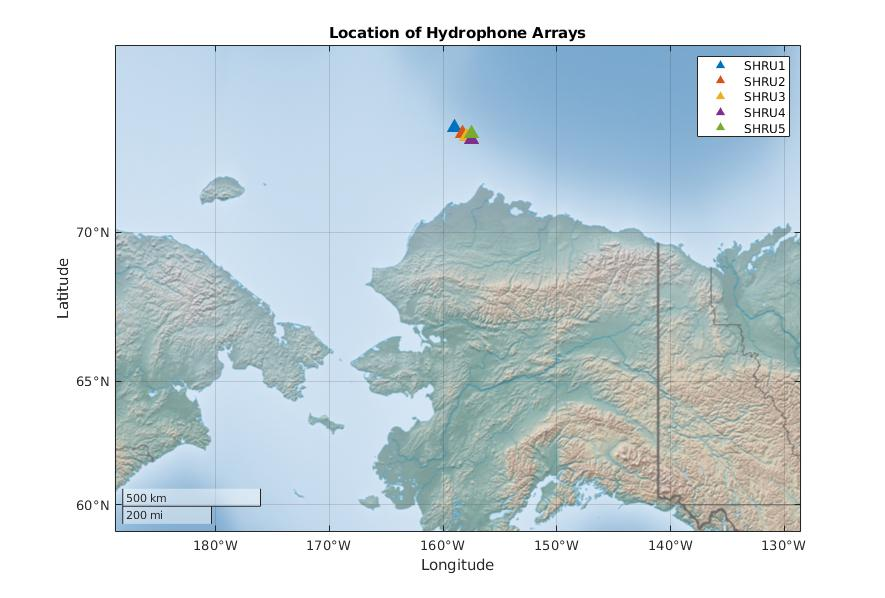
\includegraphics[scale=0.5]{Figures/west_bigmap.jpg}
\caption{Location of SHRU(s) on the Chukchi Shelf}
\label{fig_location}
\end{figure}


As the Canada Basin is an area of particular oceanographic interest, other experiments were ongoing in the region during CANAPE. The University of Delaware's oceanography moorings were also deployed on the shelf, contributed to the overall understanding of the region. Temperature profiles from this experiment helped verify the presence of the Beaufort Duct. \footcite[]{ballard2020temporal} An experiment in DW-CANAPE did create signal interference in the collection of noise by CANAPE, but were rejected in the data processing. \footcite[]{Bonnel2021} 


%%%%%%%%%%%%%%%%%%%%%%%%%%%%%%%%%%%%%%%%%%%%%%%%%%%%%%%%%%%%%%
\section{Data}

\subsection{Acoustic Data Collection} \label{intro_data_col}

\subsubsection{CANAPE Sources}
Acoustic data for this analysis came from SHRU5 and SHRU1 which were 50 km apart; \autoref{sec_probsnstat} contains only SHRU5 data while \autoref{chap_spacial} includes both SHRU(s). Each of the SHRU(s) were placed in the Beaufort Duct with channels 2.5 m apart, ranging from 163 to 170.5 m. The deepest channel at 170.5 m  was used for SHRU5 and the 163 m channel was used at SHRU1. The sampling rate of the SHRU(s) was $f_{s}=3906.2 Hz$ and was recorded continuously through the entire time period. This significant quantity of raw data was then transformed into acoustic products like ambient noise levels. 


\subsubsection{Processing of Acoustic Data}
In order to compute the estimated ambient noise levels, this project assumes the construction of ambient noise to be the coinciding levels of background sound and transient noise. Acoustic data was put in the spectral domain and power spectral densities (dB re 1 $\mu Pa^{2}/Hz$) produced. Then, Ambient Noise Levels (ANL) in dB re 1 $\mu Pa^{2}/Hz$ were created \footcite[]{carey2011ocean} by manually removing data containing transient signals \footcite[]{roth2012underwater}. A short description of the processing done on the CANAPE data is as follows.

The method used to create this ANL analysis derives from a previous study of ambient noise \footcite[]{bazile2013under} by an author of a CANAPE preliminary study\footcite[]{Bonnel2021}. Acoustic data was divided into non-overlapping 7 minute snapshots and then a short time Fourier transform (STFT) was performed with a sliding window of 62.5 ms and 50\% overlap. This short window has a low frequency resolution around 15 Hz but is deemed suitable for the bands of frequency analyzed. It rejects short transient signals less than a few minutes long, which removes the interference of other experimental sources mentioned in \autoref{intro_canape}. ANL is then computed using the 15th percentile of each frequency bin \footcite[]{huillery2008description}, and this process is repeated on every snapshot. Therefore, the resulting ambient noise dataset has an entry for every 7 minutes.

% Following Bartlett's method of the averaged periodogram \footcite[]{bartlett1948smoothing}, a PSD estimate was calculated using the average of the square moduli from the STFT. Long-term spectral average (LTSA) in $\mu Pa^{2}/Hz$

These ambient noise datasets were computed for 50 -1900 Hz across the whole time period. Each frequency band is 50 Hz wide and centered on frequencies from 50 to 1900, 50 Hz apart, for a total of 39 frequency bands. The range was chosen as the original sampling rate ($f_{s}$) of the SHRU(s) is  3906.2 Hz; by the Nyquist sampling frequency, the maximum reliable frequency that can be analysed is 1951.

%%%%%%%%%%%%%%%%%%%%%%%%%%%%%%%%%%%%%%%%%%%%%%%%%%%%%%%%%%%%%%%%%%%
\subsection{Environmental Data} \label{intro_env_info}

Assuming that the ambient noise had mainly environmental drivers, especially under ice, data was acquired for primary environmental factors. In addition the presence of ice coverage helped to delineate the acoustic environments for comparison during analysis. Since part of the focus was on the effects of the Beaufort Duct on the soundscape, determining when it was present greatly mattered.
%%%%%%%%%%%%%%%%%%%%%%%%%%%%%%%%%%%%%%%%%%%%%%%%%%%%%%%%%%%%%%%%%%%
\subsubsection{Ice Coverage} \label{intro_env_ice_cov}

Ice coverage (IC) was considered at the acoustic receiver location, as its influence on the duct would be most felt there. IC data originated from the Integrated Climate Data Center \footcite[]{kaleschke2001ssm} and is derived from the Special Sensor Microwave Imager (SSM/I), a remote sensor. The dataset is created using the ARTIST Sea Ice algorithm \footcite[]{spreen2008sea}. It has a daily temporal resolution and a spatial resolution of 12.5 km x 12.5 km. To reduce the influence of weather variations, ICDC applies a 5 day median filter \footcite[]{kern2010climatology}. IC data is a percentage of the area covered in ice at a grid point in space. These ice coverage percentages were then used to denote environmental time periods.

\subsubsection{Ice Drift} \label{intro_env_ice_dri}

Data for ice drift motion (IDM) came from the Ocean and Sea Ice Satellite Application Facility (OSISAF)\footcite[]{osisaf_data} of the European Organisation for the Exploitation of Meteorological Satellite (EUMETSAT) \footcite[]{osisaf_man} and the National Snow and Ice Data Center (NSIDC) \footcite[]{Tschudi2019polar}. IDM data has a spatial resolution of 25 km x 25 km and daily temporal resolution. Data comes from another microwave sensor and an algorithm that merges information from multiple sensors. The 2D vector of points across the whole Arctic are used in cm/s, though this analysis reduces it down to one dimension of km/day for ANL comparison. 

%%%%%%%%%%%%%%%%%%%%%%%%%%%%%%%%%%%%%%%%%%%%%%%%%%%%%%%%%%%%%%%%%%%
\subsection{Three Acoustic Environments} \label{intro_env_split}

Based on data from the \autoref{intro_env_ice_cov}, acoustic data can be separated intro three time segments critical to this study. Points of IC <15\% were deemed 'no ice' and point >85\% were deemed ice covered. The Beaufort duct was assumed to be present from the beginning to the middle of the ice covered period, up until approximately March 8, 2017. \footcite[]{ballard2020temporal} Intermediate values of ice coverage were omitted, and the time periods they covered cut out (November 8-23, 2016 and June 22- July 12, 2017).

For this analysis, the data is split by time into three acoustic environments:
\begin{enumerate}
    \item{'ice with duct': occurs when there is ice present and the Beaufort duct is present. From November 23, 2016 to March 8, 2017}
    \item{'ice without duct': occurs when there is ice present but the Beaufort duct does not exist. From March 9, 2017 to June 22, 2017.    }
    \item{'no ice': occurs when there is no ice or less than <15\% of ice. This environmental time period covers October 22, 2016-November 8, 2018 to June 30,2017-July 12, 2017. The environmental condition of 'no ice' also means that there is no duct.}
\end{enumerate}

These environmental naming conventions are particularly used in the probability and statistics analysis of \autoref{sec_probsnstat} to compare the ambient noise between environments. Occasionally, the moniker 'ice' is used to refer to both 'ice with duct' and 'ice without duct'. The spacial analysis in \autoref{chap_spacial} focuses only on the environment when ice is present, and so encompasses both the 'ice with duct' and 'ice without duct' environments which go from December 1, 2016 to May 30, 2017. 


%%%%%%%%%%%%%%%%%%%%%%%%%%%%%%%%%%%%%%%%%%%%%%%%%%%%%%%%%%%%%%%%%%%
\section{Statistic and Spacial Analysis}

The the chapters the follow, acoustic data will be examined through two different lenses: statistical parameters in \autoref{sec_probsnstat} and spacial correlation in \autoref{chap_spacial}. As methods the for these analyses differ, separate explanations for each will be presented. Through these chapters, we see that the Beaufort Duct raises ambient noise below 1000 Hz, that ANL is highly related across frequencies, and that IDM and ANL correlate through time.

The effects of climate change may mean that eventually there may only be the two environments 'ice with duct' and 'no ice'. Beyond that, the singular ice-less Arctic environment threatens the stability of the region. Knowing the effects and causes of the changes to the Arctic acoustic soundscape prior to their constant presence could be important for future operations and implications on life there. 

% how does one end an introduction??
%%%%%%%%%%%%%%%%%%%%%%%%%%%%%%%%%%%%%%%%%%%%%%%%%%%%%%%%%%%%%%%
% end of introduction